
\section{Overview}
\subsection{Human Action Recognition}
\begin{frame}{Human Action Recognition}
    Human action recognition (HAR) can be divided into action classification and action detection.

    \begin{enumerate}
        \item<1-> Action classification is the analysis of a segmented video containing only a single action that must be classified into a defined action category (early).
              \only<1>{
                  \begin{figure}[htp]
                      \centering
                      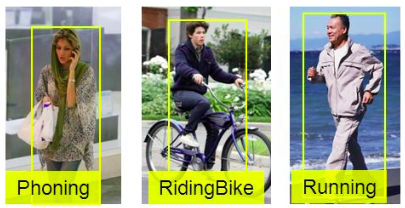
\includegraphics[width=0.6\textwidth]{images/v1survey/action-classification.png}
                      \caption{Action classification}
                      \label{fig:action-classification}
                  \end{figure}
              }
        \item<2-> Action detection detects the start and end times of each action in the video, locates their position in space, and identifies the action category (more challenging).
              \only<2>{
                  \begin{figure}[htp]
                      \centering
                      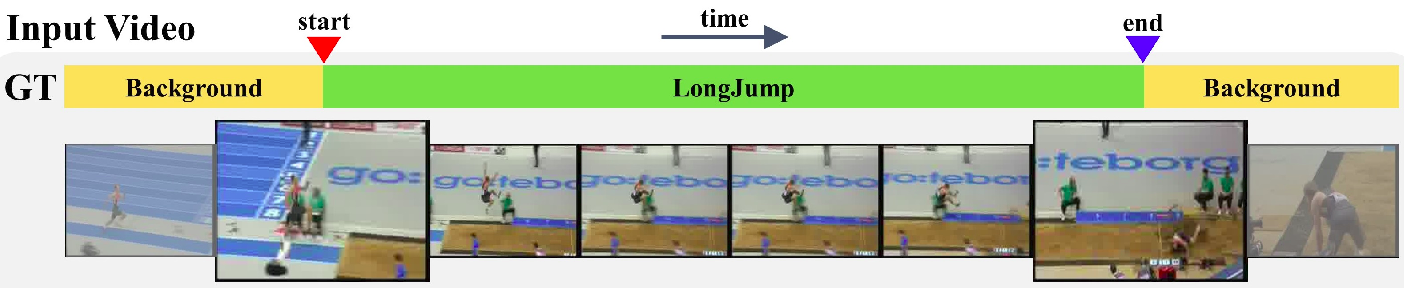
\includegraphics[width=0.8\textwidth]{images/v1survey/action-detection.jpg}
                      \caption{Action detection}
                      \label{fig:action-dectection}
                  \end{figure}
              }
    \end{enumerate}


\end{frame}

\begin{frame}{Human Action Recognition}
    Techniques can be categorized into the following four classes of action semantics from low to high:
    \begin{itemize}
        \item Primitive action recognition (waving, lifting a foot, bending).
        \item Single-person action recognition (walking, punching, jumping).
        \item Interaction recognition (playing an instrument, carrying a knife).
        \item Group action recognition (parade, group meeting).
    \end{itemize}
\end{frame}

\subsection{Applications of HAR}
\begin{frame}{Applications of HAR}
    \begin{figure}[htp]
        \centering
        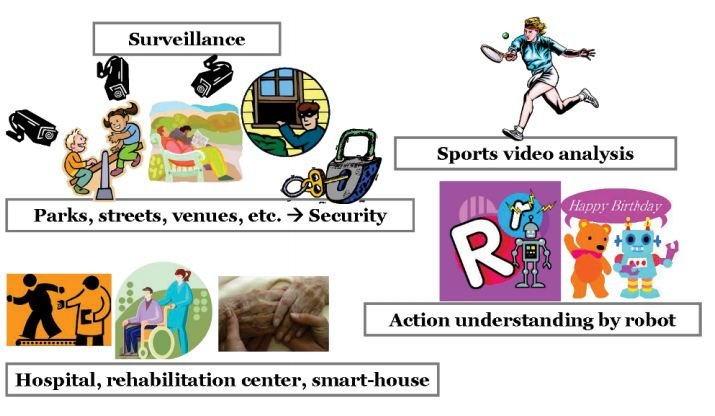
\includegraphics[width=0.7\textwidth]{images/v1survey/application.png}
        \caption{Applications}
        \label{fig:applications}
    \end{figure}
\end{frame}

\section{Type of Dataset}
\begin{frame}{Type of Dataset}

    Most reviews of human action recognition are limited to approaches based on specific data: RGB, Skeleton, Depth \cite{shahroudy2016ntu}.

    \begin{multicols}{2}
        \begin{figure}[htp]
            \centering
            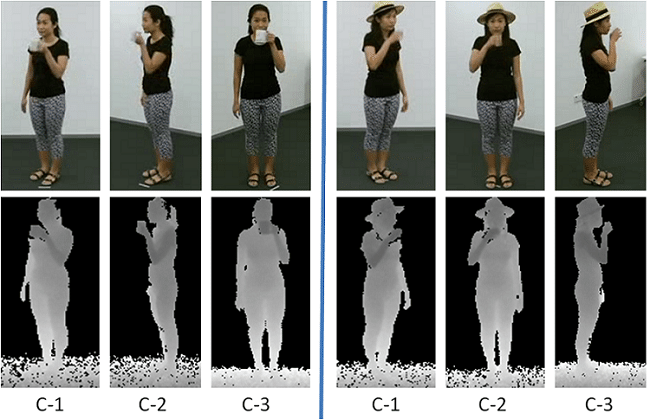
\includegraphics[height=4cm]{images/v1survey/depth_data_ex.png}
            \caption{Depth data}
            \label{fig:depth_data_ex}
        \end{figure}
        \begin{figure}[htp]
            \centering
            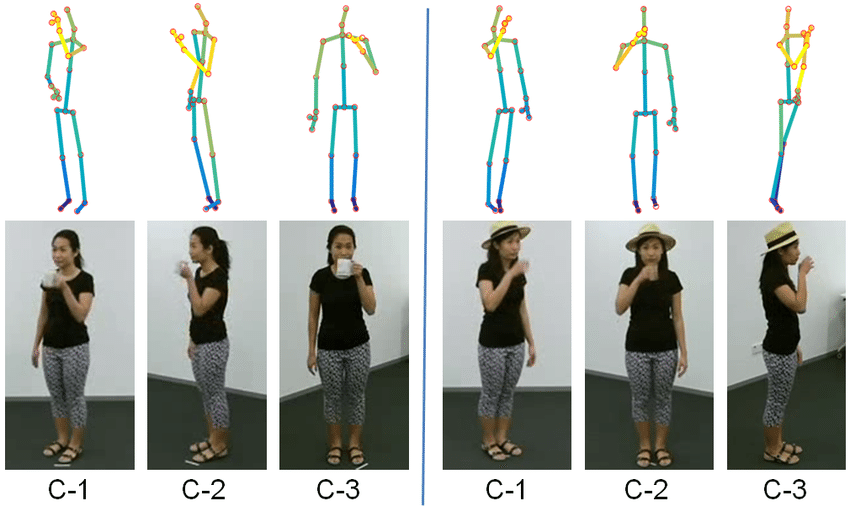
\includegraphics[height=4cm]{images/v1survey/skeleton_data_ex.png}
            \caption{Skeleton data}
            \label{fig:skeleton_data_ex}
        \end{figure}
    \end{multicols}
\end{frame}

\section{Feature representation}
\subsection{Handcrafted Action Features}
\begin{frame}{Handcrafted Action Features (RGB)}
    \begin{enumerate}
        \item<1-> Spatiotemporal volume-based action representation methods (\href{https://web.cse.ohio-state.edu/~davis.1719/CVL/Research/MHI/mhi.html}{motion history image, motion energy image}) \cite{li2011human}.
              \only<1>{
                  \begin{figure}[htp]
                      \centering
                      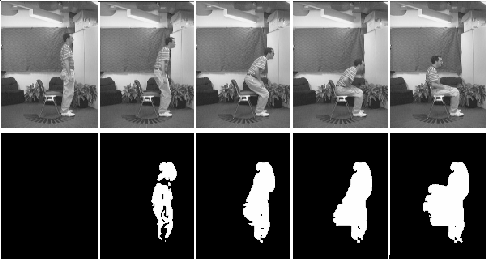
\includegraphics[height=2.25cm, width=10cm]{images/v1survey/mei.png}
                      \caption{Motion history image}
                  \end{figure}
                  \begin{figure}[htp]
                      \centering
                      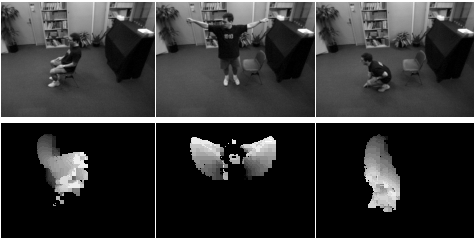
\includegraphics[height=2.25cm, width=10cm]{images/v1survey/mhi.png}
                      \caption{Motion energy image}
                  \end{figure}
              }
              % [Global features] The camera is fixed  -> background subtraction techniques
              % -> shape information (silhouettes and contours) -> key template matrix -> matching
        \item<2-> STIP-based methods (Feature descriptors: SIFT, HOG) \cite{nguyen2014stap}, \cite{dalal2005histograms}.
              \only<2>{
                  \begin{figure}[htp]
                      \centering
                      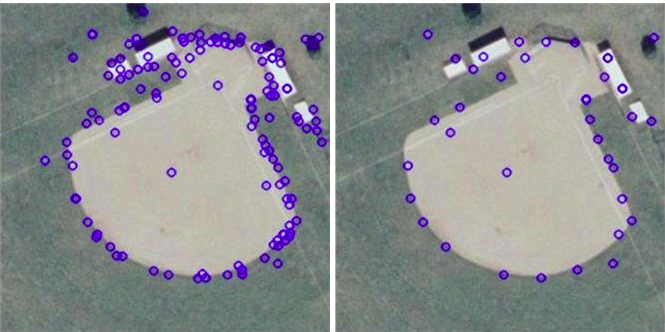
\includegraphics[width=0.6\textwidth]{images/v1survey/sift.png}
                      \caption{Scale-invariance feature transform}
                  \end{figure}
              }
              % [Local features] key region of movement change.
        \item<3-> Action representation methods based on the trajectory of skeleton joints.
              % tracking path of key points or the joints in the human skeleton
              \only<3>{
                  \begin{figure}[htp]
                      \centering
                      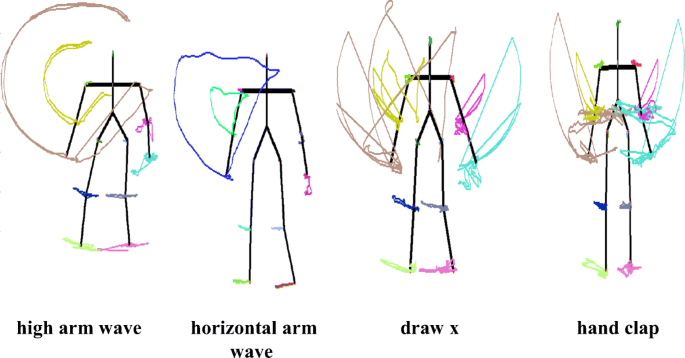
\includegraphics[width=0.5\textwidth]{images/v1survey/joins-trajectory.png}
                      \caption{Scale-invariance feature transform}
                  \end{figure}
              }
    \end{enumerate}
\end{frame}

\subsection{Methods Based on Deep Learning}
\begin{frame}{Methods Based on Deep Learning}
    \begin{itemize}
        \item In recent years, the application of deep learning to computer vision has received considerable attention.
        \item Many deep learning-based action representation methods have been proposed in the field of human action recognition
              \begin{enumerate}
                  \item 3D convolutional networks.
                  \item Two-stream convolutional networks.
                  \item Long short-term memory (LSTM).
                  \item Graph convolutional network.
              \end{enumerate}
    \end{itemize}
\end{frame}

\begin{frame}{3D convolutional networks}
    \begin{figure}[htp]
        \centering
        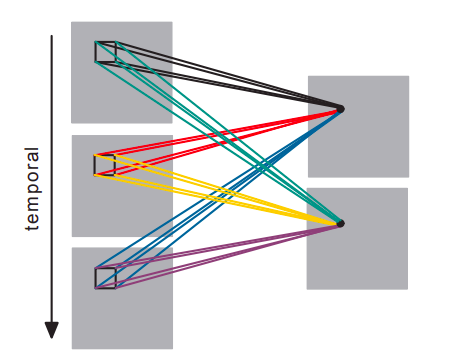
\includegraphics[width=0.5\textwidth]{images/v1survey/3d-cnn.png}
        \caption{3D convolutional networks}
    \end{figure}
\end{frame}

\begin{frame}{Two-stream convolutional networks}
    \begin{figure}[htp]
        \centering
        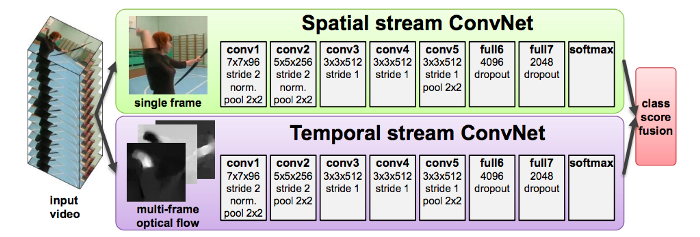
\includegraphics[width=\textwidth]{images/v1survey/2-stream-cnn.png}
        \caption{Two-stream convolutional networks}
    \end{figure}
\end{frame}

\begin{frame}[allowframebreaks]
    \frametitle{Long short-term memory (LSTM)}
    \begin{figure}[htp]
        \centering
        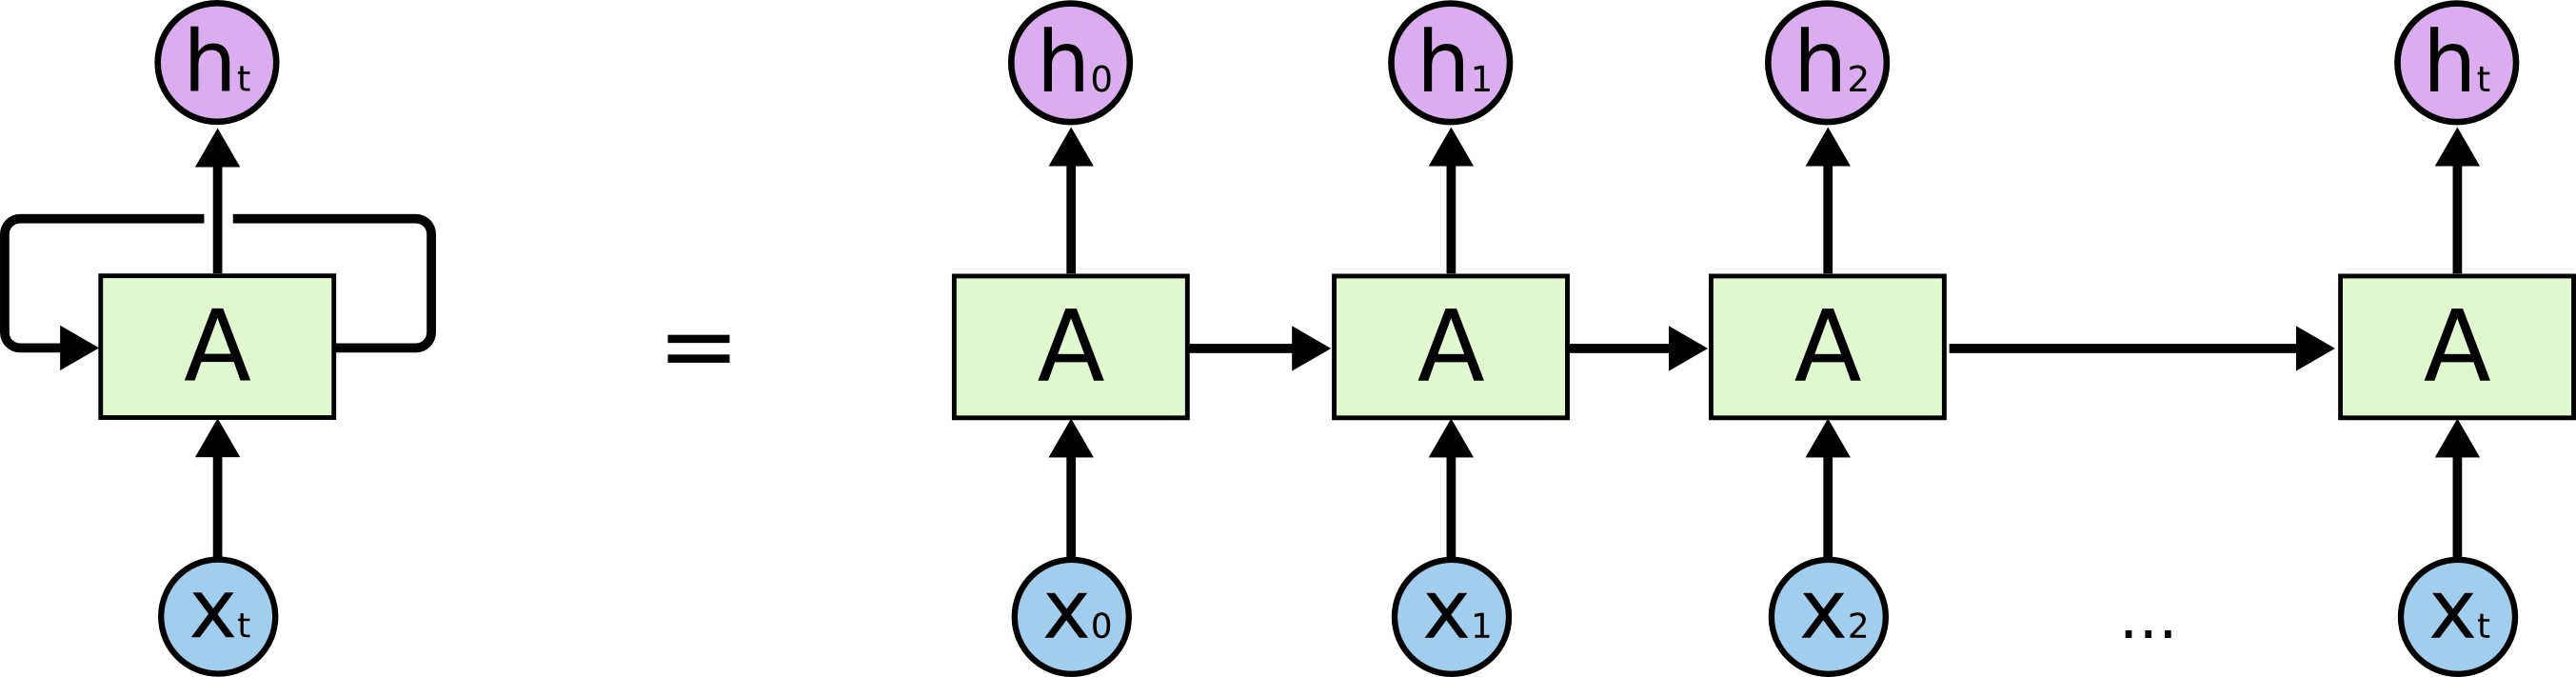
\includegraphics[width=\textwidth]{images/v1survey/RNN-unrolled.png}
        \caption{RNN}
    \end{figure}
    \begin{figure}[htp]
        \centering
        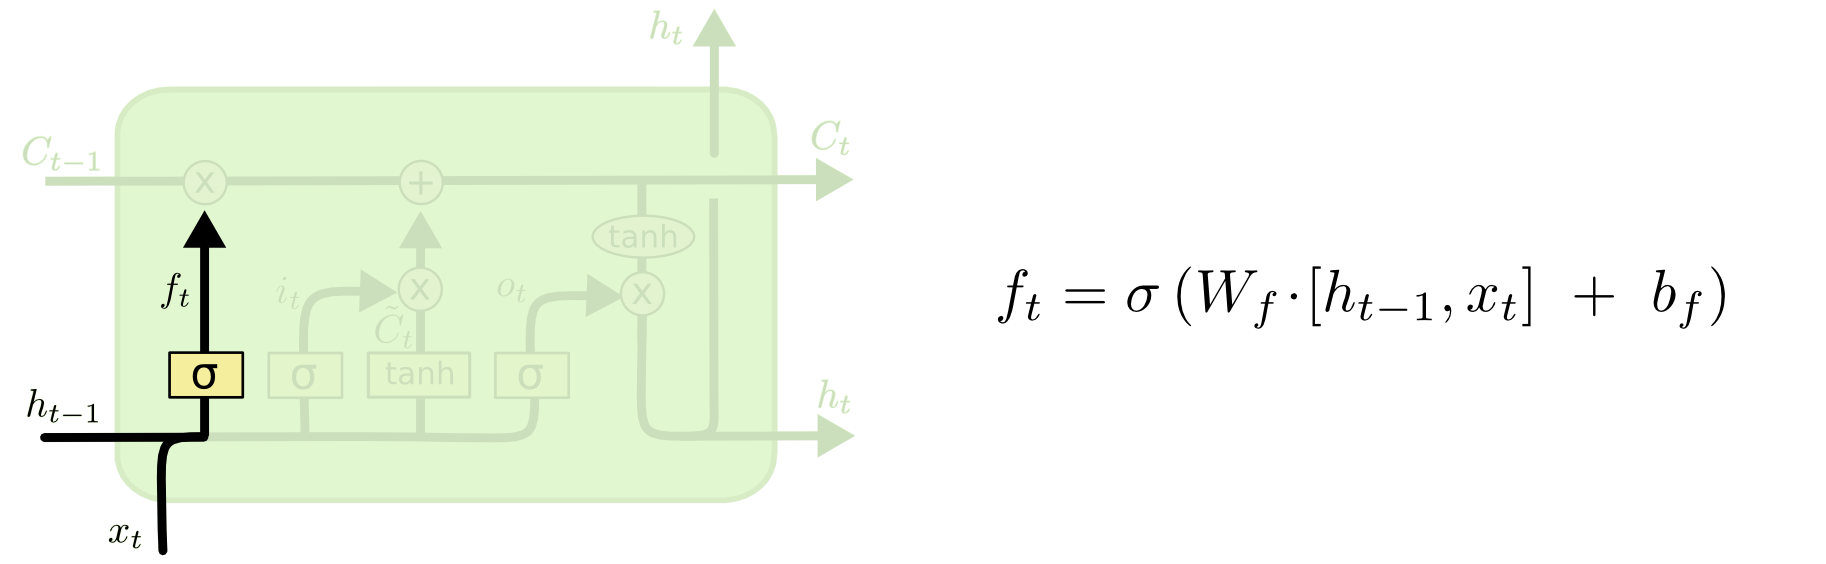
\includegraphics[width=\textwidth]{images/v1survey/LSTM-1.png}
        \caption{Forget gate layer}
    \end{figure}
    \begin{figure}[htp]
        \centering
        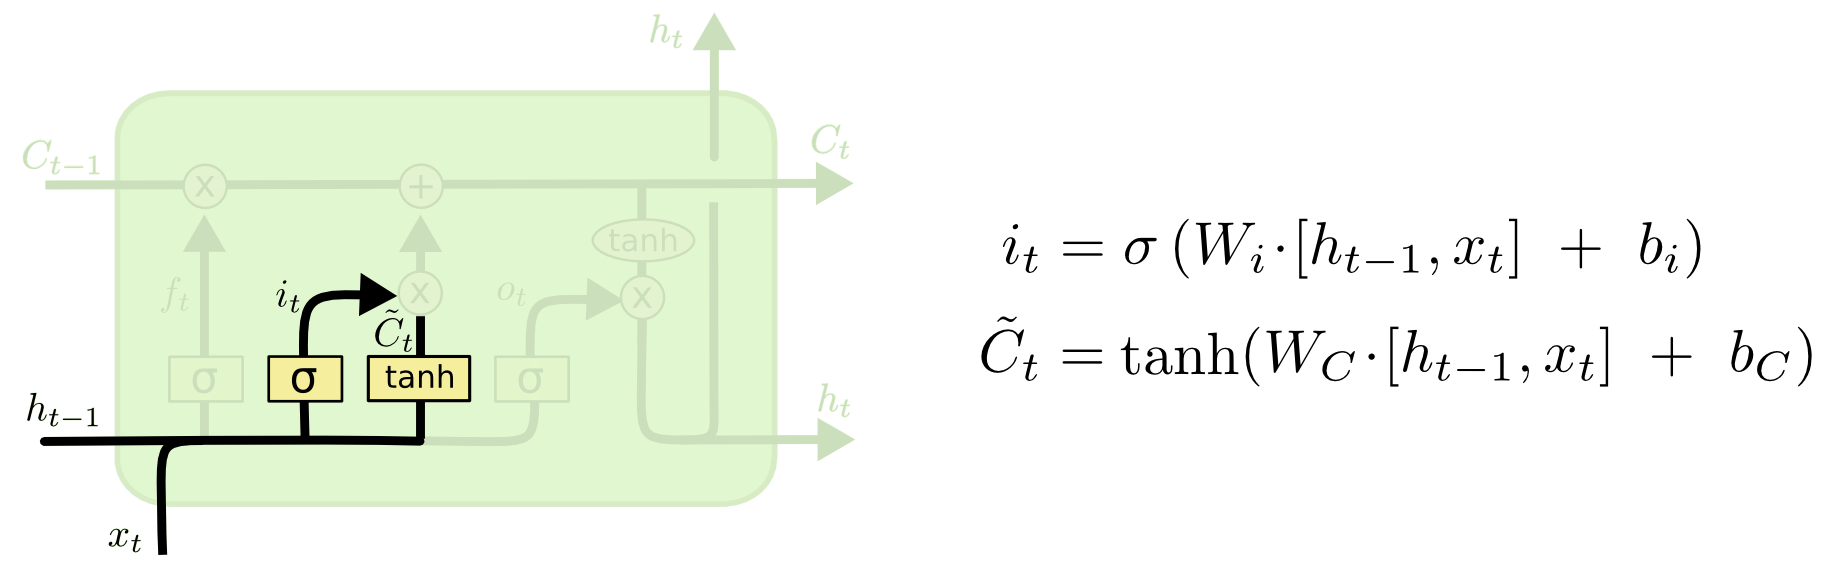
\includegraphics[width=\textwidth]{images/v1survey/LSTM-2.png}
        \caption{Input gate layer}
    \end{figure}
    \begin{figure}[htp]
        \centering
        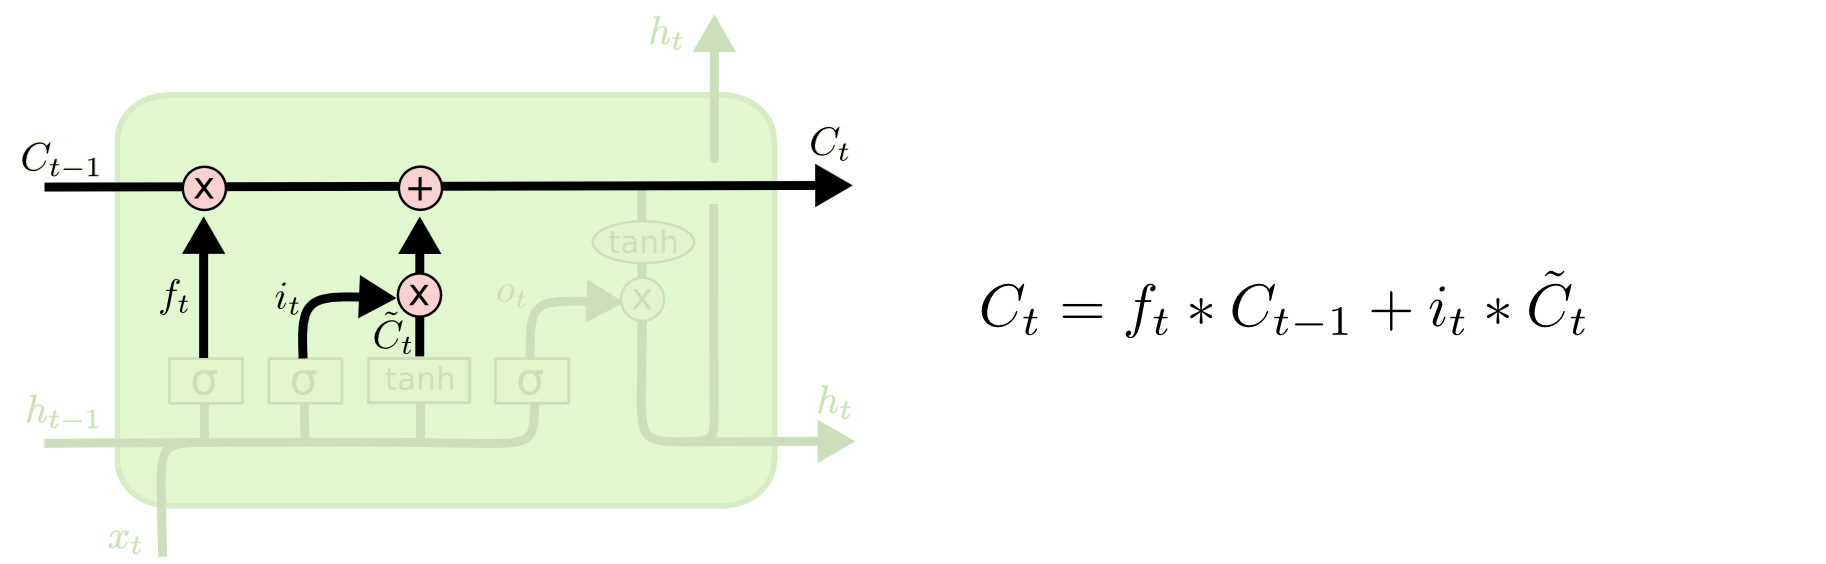
\includegraphics[width=\textwidth]{images/v1survey/LSTM-3.png}
        \caption{Update gate layer}
    \end{figure}
    \begin{figure}[htp]
        \centering
        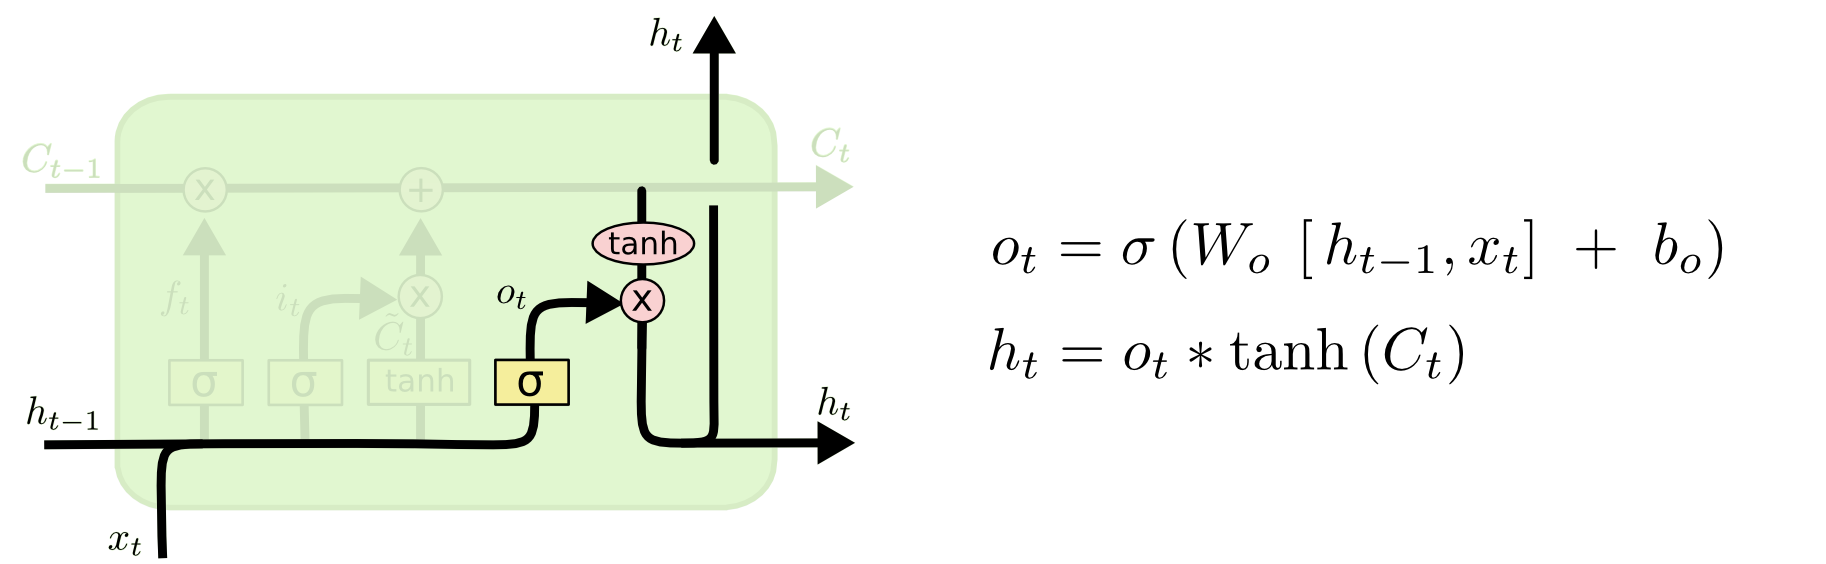
\includegraphics[width=\textwidth]{images/v1survey/LSTM-4.png}
        \caption{Output gate layer}
    \end{figure}
\end{frame}

\subsection{Graph-based machine learning}

\begin{frame}{Graph-based machine learning}
    \begin{figure}[htp]
        \centering
        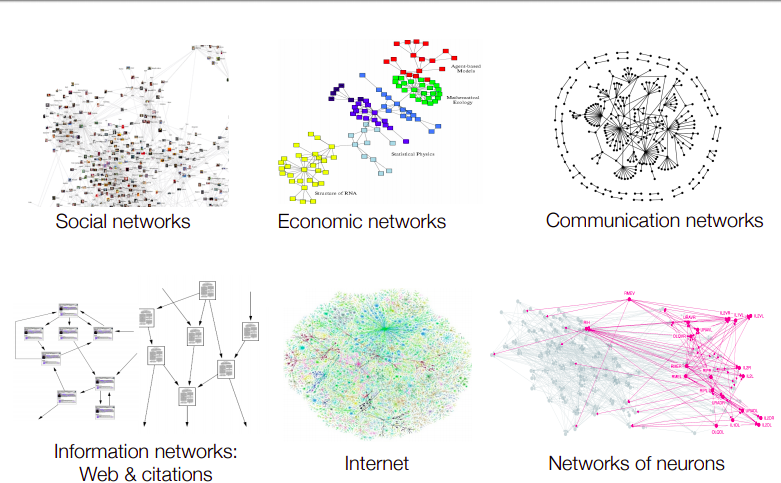
\includegraphics[width=0.7\textwidth]{images/v1survey/real-graph.png}
        \caption{Application}
        \label{fig:application}
    \end{figure}
\end{frame}

\begin{frame}{Graph-based machine learning}
    \begin{itemize}
        \item G(V, E) ~ Graph, Network, System.
        \item V Vertices ~ Nodes, Objects.
        \item E Edges ~ Link, Interaction.
    \end{itemize}
    \begin{figure}[htp]
        \centering
        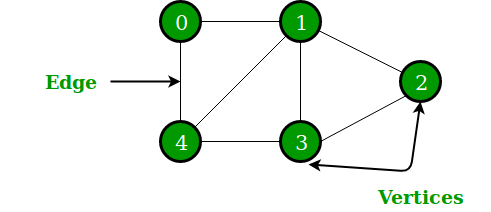
\includegraphics[width=0.7\textwidth]{images/v1survey/graph.png}
        \caption{Graph}
        \label{fig:graph}
    \end{figure}
\end{frame}

\begin{frame}{Graph-based neural network}
    \begin{block}{What is non-Euclidean data?}
        The shortest path between 2 points isn't necessarily a straight line.
    \end{block}

    \begin{figure}[htp]
        \centering
        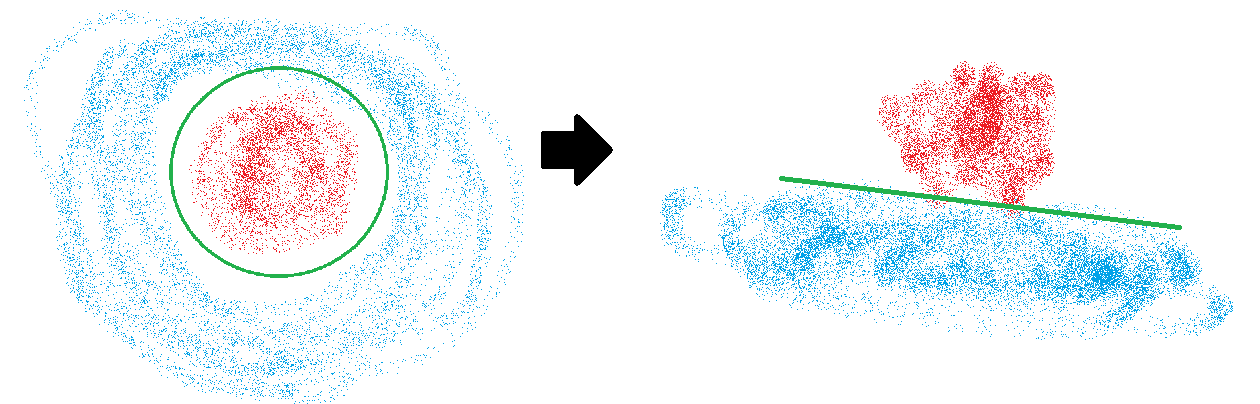
\includegraphics[width=0.8\textwidth]{images/v1survey/concrete_plot.png}
        \caption{Concrete examples}
    \end{figure}
\end{frame}

\begin{frame}{Graph-based neural network}
    \begin{figure}[htp]
        \centering
        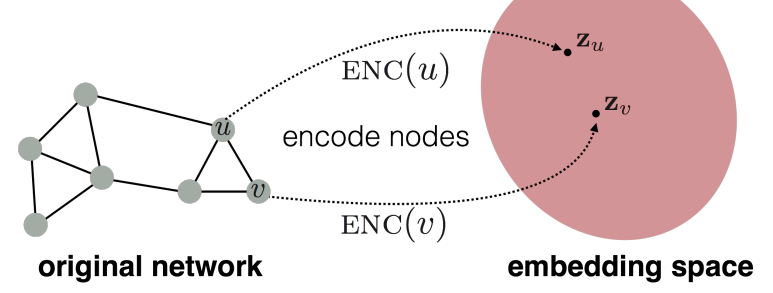
\includegraphics[width=0.8\textwidth]{images/v1survey/euclid_space.png}
        \caption{Embedding}
    \end{figure}
\end{frame}

\begin{frame}{Graph-based neural network - Word embeeding}
    \begin{figure}[htp]
        \centering
        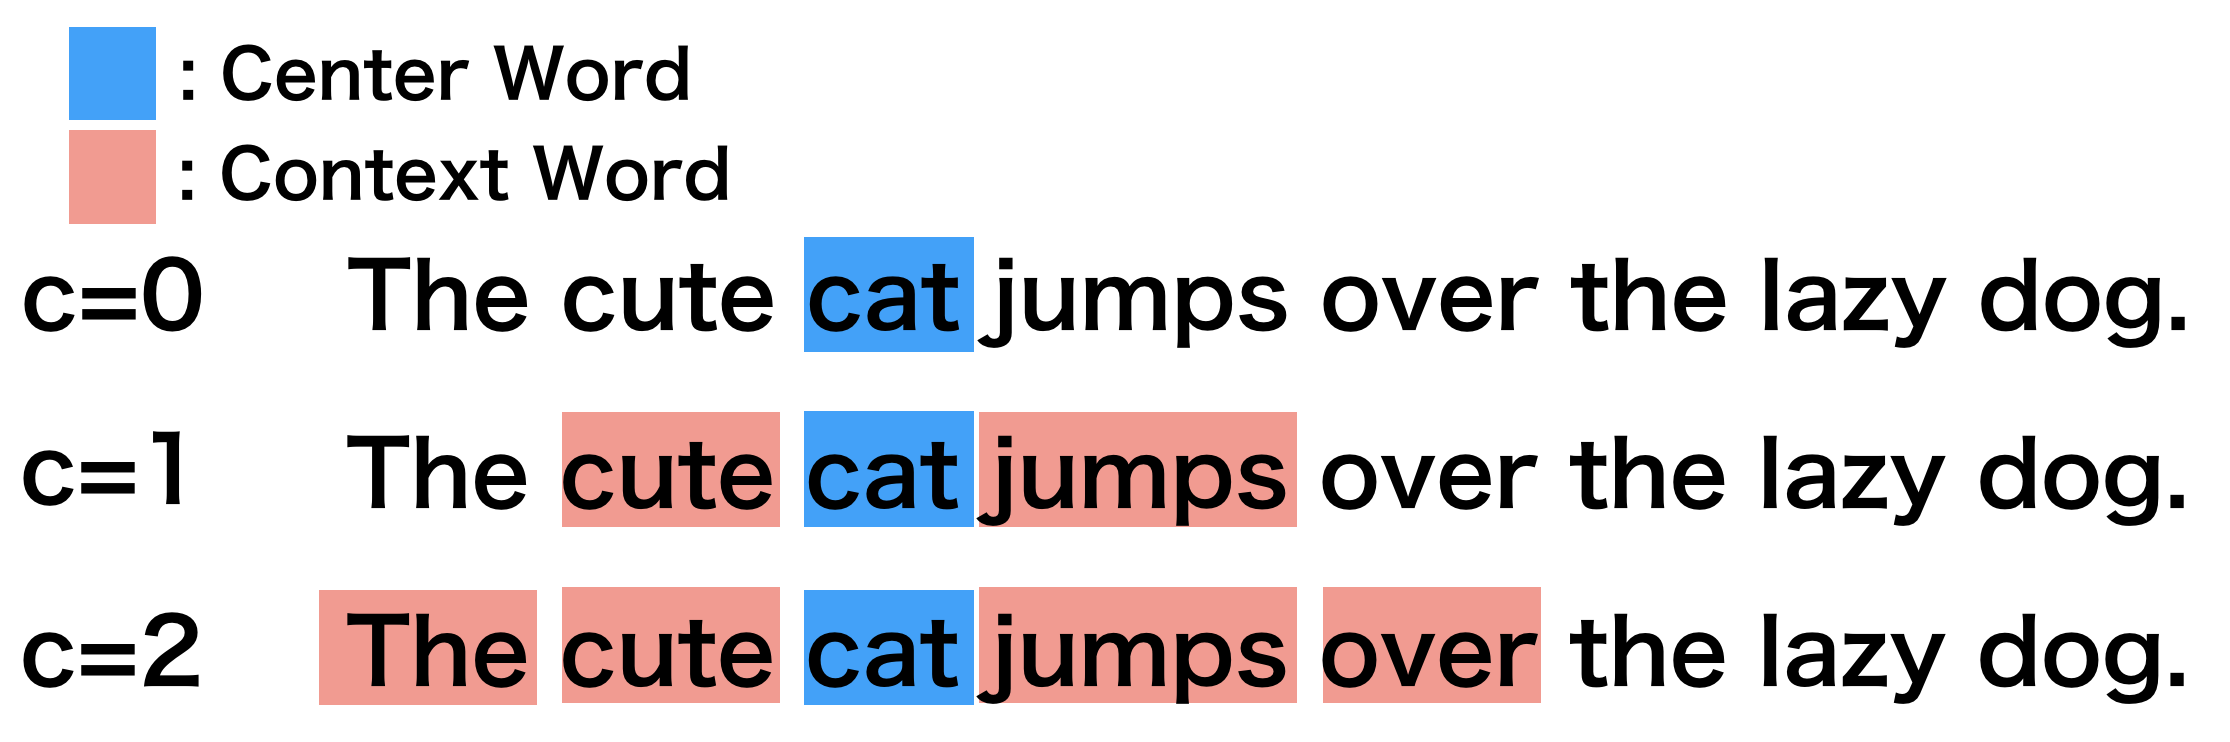
\includegraphics[width=0.8\textwidth]{images/v1survey/context-word.png}
        \caption{Context word}
    \end{figure}
\end{frame}

\begin{frame}{Graph-based neural network - CBOW}
    \begin{multicols*}{2}
        \begin{figure}[htp]
            \centering
            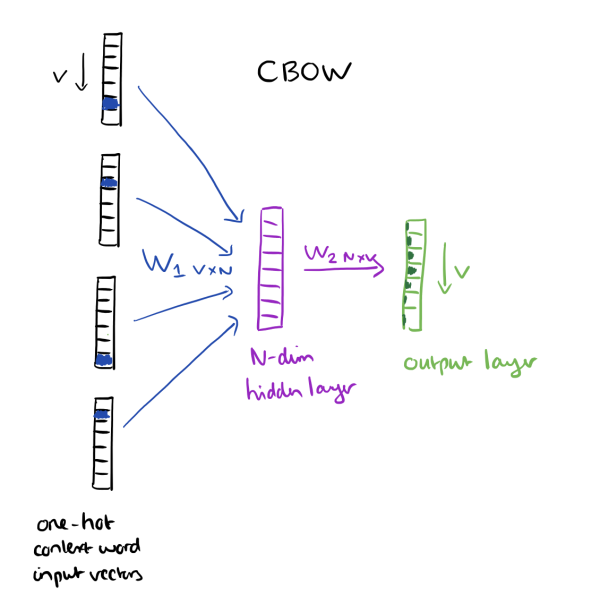
\includegraphics[width=0.4\textwidth]{images/v1survey/cbow.png}
            \caption{CBOW}
        \end{figure}

        \begin{figure}[htp]
            \centering
            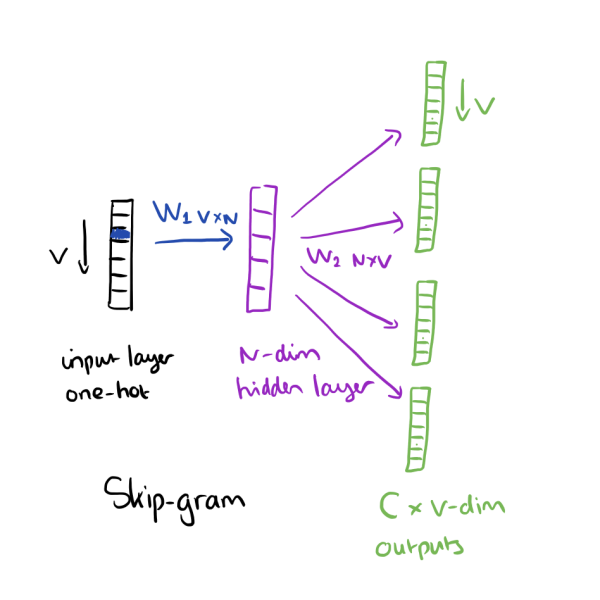
\includegraphics[width=0.4\textwidth]{images/v1survey/skip-gram.png}
            \caption{Skip-gram}
        \end{figure}
    \end{multicols*}
\end{frame}

\begin{frame}{Graph-based neural network - DeepWalk}
    DeepWalk (Perozzi et al., 2014) is introduced to learn node embeddings via a random walk and word2vec (Mikolo et al., 2013) word2vec algorithm.
    \begin{figure}[htp]
        \centering
        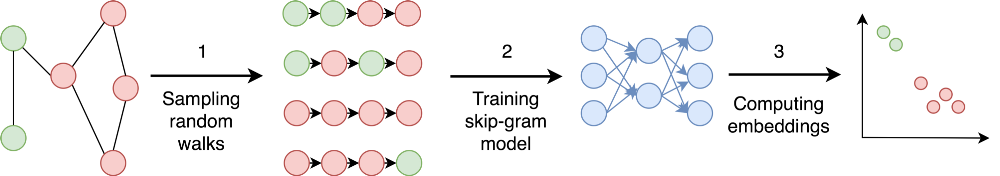
\includegraphics[width=\textwidth]{images/v1survey/deepwalk.png}
        \caption{DeepWalk}
    \end{figure}
\end{frame}

\begin{frame}{Graph-based neural network - Node2Vec}
    \begin{figure}[htp]
        \centering
        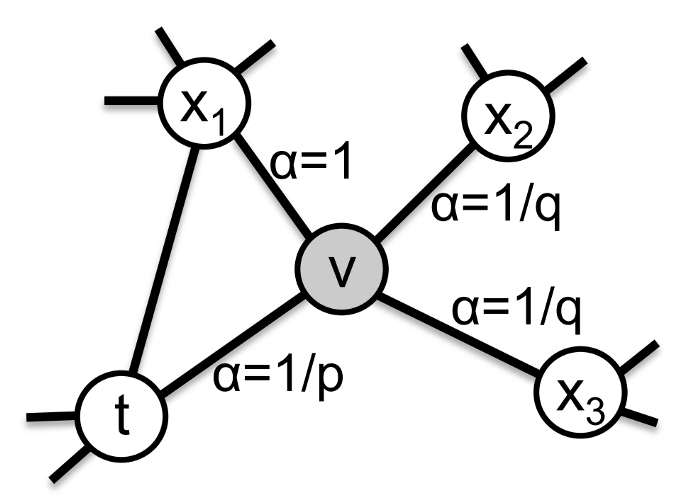
\includegraphics[width=0.6\textwidth]{images/v1survey/p-q-param.png}
        \caption{p q param}
    \end{figure}
\end{frame}